\scanpage{61}
\[
0\leq i\leq j\leq n-1\qquad
\rho_{ij}=L_{j-i+2}(\beta_i,\beta_{i+1},\ldots,\beta_j)
=L_{\unsure{j-i+1}}(\beta_j,\beta_{j-1},\ldots,\beta_i)
\]
\margin{\deleted{\(\widetilde\rho_{ij}=\frac12\rho_{ij}\)}}
\deleted{\(\unsure{a}\)}
\[
\rho=\rho_{0,n-1},\quad \sigma=\rho_{1,n-1},\quad
\sigma'=\rho_{0,n-2},\quad \gamma=\rho_{1,n-2}
\]
On pose aussi \(\rho_{i,i-1}=2,\quad\rho_{i,i-2}=1\)
\margin{\(\rho'_{ji}=\rho_{ij}\quad(j\geq i\)}
\[
\boxed{a_i^*=a'_{i+1}+2a'_{i+2}
+\cdots\rho_{i+1,i+j}a'_{i+j+2}+\cdots+\rho_{i+1,n-1}a'_{n+1}}
\qquad -1\unsure{\leq|<}i\leq n
\]
\deleted{\(a_j^*=\)}
en particulier pour \(i=-1,\ i=0\)
\[
\left\{\begin{aligned}
a_{-1}^*&=\Pi'=a'_0+2a'_1+
\overbrace{\rho_{0,0}}^{4-\beta_0=2-\alpha_0}a'_2+
\rho_{0,1}a'_3+\cdots+
\overbrace{\rho_{0,n-2}}^{\sigma'}a'_n+
\overbrace{\rho_{0,n-1}}^\rho a'_{n+1}\\
a_0^*&=-\Psi(a_{-1})=-\Psi(s_0)
=a'_1+2a'_2+\rho_{1,1}a'_3+\cdots+
\overbrace{\rho_{1,n-2}}^\gamma a'_n+
\overbrace{\rho_{1,n-1}}^\sigma a'_{n+1}\\
[\,a_1^*&=a'_2+2a'_3+\rho_{22}a'_{\unsure{3|4}}+\mathbin{-}
+\rho_{2,n-2}a'_n+\rho_{2,n-1}a'_{n+1}\\
&\mathbin{-}\mathbin{-}\\
a_{n-2}^*&=a'_{n-1}+2\unsure{a_n|a'_n}+
\overbrace{\rho_{n-1,n-1}}^{4-\beta_{n-1}=2-\alpha_{n-1}}a'_{n+1}\\
a_{n-1}^*&=a'_n+2a'_{n+1}\\
a_n^*&=a'_{n+1}
\end{aligned}\right.
\]
\figure{\begin{tikzpicture}
\draw[->] (0,0) .. controls (1,0.2) and (3,0.3) .. (3.6,0.1)
.. controls (4,0.2) and (4,3.2) .. (4,5.6);
\end{tikzpicture}}
\figure{\begin{tikzpicture}
\node[draw,ellipse,inner sep=12pt] {\(
\widetilde\rho_{ij}=
\begin{cases}
\deleted{\unsure{2}}\rho_{ij}&\text{si }j-i\ \deleted{\unsure{\text{impair}}}\text{pair}\\
\frac12\rho_{ij}&\text{si }j-i\ \deleted{\text{pair}}\inserted{\text{impair}}
\end{cases}\)};
\end{tikzpicture}}
\deleted{Dualement}
\[
\boxed{
a_j'^*=a_{j-1}^*+2a_{j-2}^*
+\rho'_{j-2,j-2}a_{j-3}^*+\mathbin{-}
+\rho'_{j-2,j-\unsure{i}}a_{j-\unsure{i}-1}^*
+\mathbin{-}+\rho'_{j-2,0}a_{-1}}
\]
\[
\left\{\begin{aligned}
a_{n+1}'^*&=\Pi=a_n+2a_{n-1}
+\underbrace{\rho'_{n-1,n-1}}_{4-\beta_{n-1}=2-\alpha_{n-1}}a_{n-2}
\mathbin{-}+
\overbrace{\rho'_{n-1,1}}^\sigma a_0+
\overbrace{\rho'_{n-1,0}}^\rho a_{-1}\\
a_n'^*&=-\Psi'(a'_{n+1})=a_{n-1}+2a_{n-2}
+\underbrace{\rho'_{\unsure{n-1|n-2},n-2}}_{4-\beta_{n-2}=2-\alpha_{n-2}}a_{n-3}
+\mathbin{-}+
\overbrace{\rho'_{n-2,1}}^\gamma a_0+
\overbrace{\rho'_{n-2,0}}^{\sigma'}a_{-1}\\
&\mathbin{-}\mathbin{-}\\
a_2'^*&=a_1^*+2a_{\unsure{2|0}}+
\underbrace{\rho'_{0,0}}_{4-\beta_0=2-\alpha_0}a_{-1}\\
a_1'^*&=a_0+2a_{-1}\\
a_0'^*&=a_{-1}
\end{aligned}\right.
\qquad \boxed{\langle\Pi,\Pi'\rangle=\rho}
\]
\figure{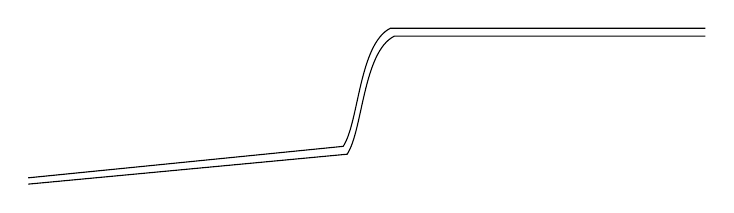
\begin{tikzpicture}
\draw (0,0)--(4,0.4).. controls (4.2,0.7) and (4.2,1.7)..(4.6,1.9)--(8.6,1.9);
\draw (0,-0.08)--(4.05,0.3).. controls (4.25,0.6) and (4.25,1.6)..(4.65,1.8)--(8.6,1.8);
\end{tikzpicture}}
\[
\left\{\begin{aligned}
\Psi(a_i)&=-(\beta_0\mathbin{-}\beta_{i-1})a'_i
&&0\leq i\leq n\\
\Psi(a_{-1})&=-a_0^*\unsure{=-|=}
[a'_1+2a'_2+\rho_{11}a'_3+\mathbin{-}\mathbin{-}
+\overbrace{\rho_{1,n-2}}^\gamma a'_n+
\overbrace{\rho_{1,n-1}}^\sigma a'_{n+1}]\\
f(a_i)&=\beta_0\mathbin{-}\beta_{i-1}&&0\leq i\leq n\\
f(a_{-1})&=0
\end{aligned}\right.
\]
\margin{\[
f(a_0)=1,\quad f(a_1)=\beta_0,\mathbin{-},\quad
f(a_n)=\beta_0\mathbin{-}\beta_{n-1}=\unsure{B|\beta}
\]}
\[
\varphi(a_i,a_{i+1})=-\deleted{\unsure{\beta_0\times}}\beta_0\mathbin{-}\beta_i
\qquad0\leq i\leq n-1
\]
\[
\Psi(\Pi)=-\sigma\Pi'\qquad
f(\Pi)=-\widetilde\sigma\widetilde\rho
\]
\mspage{60}
\mspage{60}

